\documentclass{beamer}

\usepackage{amssymb}
\usepackage{fancyvrb}
\usepackage{stmaryrd}
\usepackage{graphicx}
\usepackage{tikz}
\usefonttheme{serif}


\newcommand{\Nat}{\mathbb{N}}

\title{Data Science}%\texorpdfstring{$\mathbb{N}$}}
\subtitle{\blueit{Introduction to Machine Learning:\\
                  Random Forests, k-NN, Feature Engineering}}
\date{April 21, 2021}

\usetheme{jmct}

\usepackage{calc}

\newcommand{\textover}[3][l]{%
 % #1 is the alignment, default l
 % #2 is the text to be printed
 % #3 is the text for setting the width
 \makebox[\widthof{#3}][#1]{#2}%
 }

\newcommand{\blueit}[1]{%
  {\color{dark-lucid-blue}#1}%
}
\newcommand{\blueite}[1]{%
  \blueit{\emph{#1}}%
}
\newcommand{\redit}[1]{%
  {\color{my-magenta}#1}%
}


\newcommand{\myquote}[3]{
  ``#1''
  \vspace{3pt}
  \hrule
  \begin{flushright}
  --- \blueit{\emph{#2}}, \emph{#3}
  \end{flushright}
}

\begin{document}
	\frame {
		\titlepage
	}

\newcommand{\withwidth}[2]{%
  \makebox[\widthof{#2}][c]{#1}%
}

%%%%%%%%%%%%%%%%%%%%%%%%%%%%%%%%%%%%%%%% 
%%% Intro
%%%%%%%%%%%%%%%%%%%%%%%%%%%%%%%%%%%%%%%% 

  \frame{
    \frametitle{Goals for today}
    A quick survey of other ML methods
    \begin{enumerate}
      \item<2 -> We've looked at two very different ways to build predictive models:
      \begin{enumerate}
        \item<3 -> Linear Regressions
        \item<4 -> Decision Trees
      \end{enumerate}
      \item<5 -> What else is out there?
    \end{enumerate}
  }

  \frame{
    \frametitle{Previously, on...}
    Decisions Tress are great, but...
    \begin{enumerate}
      \item<2 -> They are very brittle (prone to over-fit)
      \item<3 -> We discussed one way of combating that (Holdout Cross Validation)
      \item<4 -> Is there any other way, specific to decision trees?
      \item<5 -> Yes, Just make more trees!
    \end{enumerate}
  }

  \frame{
    \frametitle{Random forests}
    If one DT is brittle, make a bunch of trees to do the work together.
      \begin{enumerate}
        \item<2 -> Problem: How do we make sure that they're not all brittle in the same way?
        \item<3 -> Solution (part 1): You don't use the whole dataset to train all of them.
        \item<4 -> Solution (part 2): You don't use \emph{all} of the features in the DTs
        \item<5 -> These parts are known as \blueite{baggin} and \blueite{random feature selection}
      \end{enumerate}
  }

  \frame{
    \frametitle{That's my bag}

    Bagging is short for Bootstrap Aggregation:

      \begin{enumerate}
        \item<2 -> From you dataset, sample (with replacement!) $n$ elements
        \item<3 -> For some number, $B$, of sample sets, train a DT for each $i \in B$
        \item<4 -> Now we need to Aggregate:
        \item<5 -> Thoughts on how?
        \begin{enumerate}
          \item<6 -> It depends on whether you need a classifier!
        \end{enumerate}
      \end{enumerate}
  }

  \frame{
    \frametitle{Aggregate 1: You don't need a classifier}

    For each $T_i$ we get some prediction $y_i$.

    \begin{enumerate}
      \item<2 -> For a regression, just take the average:
      \item<3 -> $\frac{1}{|B|} \sum\limits_{j \in B} y_j$
    \end{enumerate}
  }

  \frame{
    \frametitle{Aggregate 2: You do need a classifier}

    For each $T_i$ we get some prediction $y_i$.

    \begin{enumerate}
      \item<2 -> For a classifier, just treat it as a vote!
    \end{enumerate}
  }

  \frame{
    \frametitle{RAS}

    Bagging ads some randomness, let's add more\footnote{it is a \emph{random} forest, after all}

      \begin{enumerate}
        \item<2 -> For each \redit{tree}, at every split point (where you'll put a decision node):
        \begin{enumerate}
          \item<3 -> choose a \blueite{random} subset of the available attributes (features)
          \item<4 -> Use the same ``most significant'' attribute process as before, but only on that random subset.
        \end{enumerate}
        \item<5 -> This reduces the correlation \emph{between} trees!
      \end{enumerate}
  }

  \begin{frame}[fragile]
    \frametitle{Random Trees (classifier) with SKLearn:}
  
        \centering
    {\color{dark-gray}
        \begin{BVerbatim}
from sklearn.ensemble import RandomForestClassifier

classifier = RandomForestClassifier(n_estimators=N)
classifier = classifier.fit(X, Y)
        \end{BVerbatim}
  }

  \end{frame}

  \begin{frame}[fragile]
    \frametitle{Random Trees (regressor) with SKLearn:}
  
        \centering
    {\color{dark-gray}
        \begin{BVerbatim}
from sklearn.ensemble import RandomForestRegressor

classifier = RandomForestRegressor(n_estimators=N)
classifier = classifier.fit(X, Y)
        \end{BVerbatim}
  }

  \end{frame}

  \begin{frame}[fragile]
    \frametitle{Other useful parameters:}

    Both use bootstraping by default (though you can turn it off)

      \begin{enumerate}
        \item<2 -> \verb`max_depth`: How deep of a tree you'll allow
        \item<3 -> \verb`max_samples`: How many samples you'll allow for each $T$
        \item<4 -> \verb`min_samples_leaf`: How many samples needed for a leaf node to be created.
      \end{enumerate}
  \end{frame}

%%%%%%%%%%%%%%%%%%%%%%%%%%%%%%%%%%%%%%%% 
%%% k-NN
%%%%%%%%%%%%%%%%%%%%%%%%%%%%%%%%%%%%%%%% 


  \frame{
    \frametitle{The company you keep}
      What if we don't want to think too hard about what our features mean?\footnote{This is a charicature!}
      
      \begin{enumerate}
        \item<2 -> The human brain is very good at pattern matching (this is good and bad)
        \item<3 -> One way we determine what `group' something belongs to is to see what it's near!
        \item<4 -> Let's write a program to do that.
      \end{enumerate}
  }

  \frame{
    \frametitle{$k$-NN}
    First let's define a \emph{neighbor}

      \begin{enumerate}
        \item<2 -> For many types of features, we can have a notion of \blueite{distance}
        \item<3 -> Using that notion of distance we can ask questions like:
        \begin{enumerate}
          \item<4 -> Is $B$ or $C$ closer to point $A$?
        \end{enumerate}
        \item<5 -> We can ask this for every point in the dataset, for \emph{every other} point in the dataset
        \item<6 -> This can give us an \blueite{ordering} of the \redit{nearest neighbors}.
      \end{enumerate}
  }

  \frame{
    \frametitle{$k$...}

      \begin{enumerate}
        \item<2 -> When $k = 1$, we only care about the closet point.
        \item<3 -> When $k = 2$, we only care about the two closet points, and they `vote'.
        \item<4 -> When $k = 3$, we only care about the... you get it.
      \end{enumerate}
  }

  \frame{
    \frametitle{Discussion time.}
    What do we have to do in order to train this model?

      \begin{enumerate}
        \item<2 -> We only have to store the dataset in a way that let's us calculate the nearest neighbor(s)
      \end{enumerate}
  }

  \frame{
    \frametitle{Discussion time 2.}
    What do we think $k$-NN might be good for?
  }

  \frame{
    \frametitle{Let's take a look (1NN):}
    

    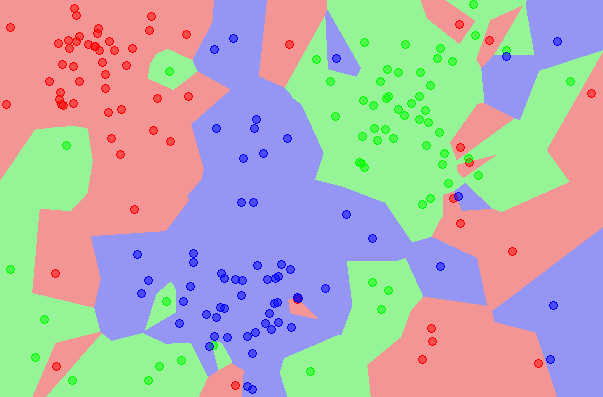
\includegraphics[width=\textwidth]{figs/Map1NN.png}
  }

  \frame{
    \frametitle{Let's take a look (5NN):}
    

    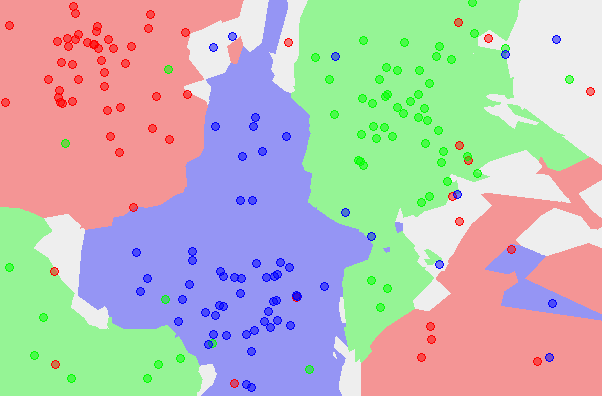
\includegraphics[width=\textwidth]{figs/Map5NN.png}
  }

  \begin{frame}[fragile]
    \frametitle{$k$-NN and SKLearn}
    You might see a pattern developing:

      \begin{enumerate}
        \item<2 -> \verb`sklearn.neighbors.KNeighborsClassifier`
        \item<3 -> Defaults to $k = 5$
        \item<4 -> You can also play with the \verb`metric` and \verb`p` parameters to change how distance is calculated (default is Euclidean distance).
      \end{enumerate}
  \end{frame}


  \frame{
    \frametitle{Feature Engineering (interaction terms)}

      \begin{enumerate}
        \item<2 -> Sometimes (as in the video for the make up lecture) we only want to add categorical terms
        \item<3 -> But sometimes we also want to add \emph{interactions} between our terms.
        \item<4 -> To the notebook!
      \end{enumerate}
  }


%%%%%%%%%%%%%%%%%%%%%%%%%%%%%%%%%%%%%%%% 
%%% Conclusion
%%%%%%%%%%%%%%%%%%%%%%%%%%%%%%%%%%%%%%%% 

  \frame{
    \frametitle{Thanks for your time!}

     :) 
  }


\end{document}
